\documentclass[10pt]{article}

\usepackage{graphicx}
\usepackage{float}
\usepackage{tocloft}
\usepackage{caption}

\renewcommand{\cftsecleader}{\cftdotfill{\cftdotsep}}

\usepackage[backend=biber, style=IEEE]{biblatex}
\addbibresource{resources/references.bib}


\begin{document}
\makeatletter

% title page
\begin{titlepage}
	\begin{center}
		\line(1,0){300}\\
		[0.32cm]
		\huge{\bfseries Federated Machine Learning}\\
		[0.16cm]		
		\line(1,0){300}\\
		[0.64cm]		
		\textsc{\LARGE A research project}\\
		[10cm]
	\end{center}
	\begin{flushright}
		\textsc{\large Karan Samani}\\
		1161081087\\
		BSc. Computer Science (Hons.)\\
		\@date
	\end{flushright}
\end{titlepage}
\cleardoublepage

% Front matter
\pagenumbering{roman}
\section*{Abstract}
\addcontentsline{toc}{section}{\numberline{}Declaration}
Federated machine learning is the idea (from Google) of anonymised machine learning (or rather deep learning). It is a way to get a Neural Network trained on everyones data, but without having direct access to everyones data.

Traditionally, a Neural Network would require a lot of data from users to train a model that is fairly accurate. But with the federated approach, the users dont have to share their data with anyone else to obtain a better overall model. Instead, they train a model locally no their own data, and then send the weights and biases of the model (the original user data cannot be recreated with these weights and biases) to a server which then averages them and sends them to you all the users. Because the weight and biases are being sent, instead of the users actual data (like their images), privacy is maintained and essentially a model is trained using anonymised data from several users.

My project is based on implementing the way in which Google does this, and then implementing several more strategies proposed by Derek and comparing their outcome. At a high level, these strategies include discarding the weights of users in certain conditions or using a weighted average of their weights and biases.\\
\clearpage
\section*{Declaration}
\addcontentsline{toc}{section}{\numberline{}Abstract}
\clearpage

\section*{Acknowledgements}
Thanks to Dr. Derek Bridge for dealing with me over the last few months, pushing me to my limits and giving support as and when required.\\\\
Thanks to the Alexander Baran-Harper's channel on YouTube where I learnt how to use use LaTeX.
\addcontentsline{toc}{section}{\numberline{}Acknowledgements}
\clearpage


% Table of content stuff
\tableofcontents
\thispagestyle{empty}
\cleardoublepage

% list of figures
\listoffigures
\addcontentsline{toc}{section}{\numberline{}List of Figures}
\cleardoublepage


% project work
\setcounter{page}{1}
\pagenumbering{arabic}


\section{Artificial Intelligence (dont know where to put this chapter}\label{sec:ai}
\subsection{What is AI?}
Artificial Intelligence can be described as the ability for a system to show “intelligence”. Intelligence, as Dr. Derek Bridge put it, is the ability for a system to act autonomously and rationally when faced with disorder, uncertainty, imprecision and intractability. A subset of AI is called Machine Learning. ML is a broad field of AI application where explicit programming is not required for the system to recognise patterns and learn. The area of Neural Networks (and Deep Learning) is the one that will be explored in this project.
\begin{figure}[H]
	\centering
	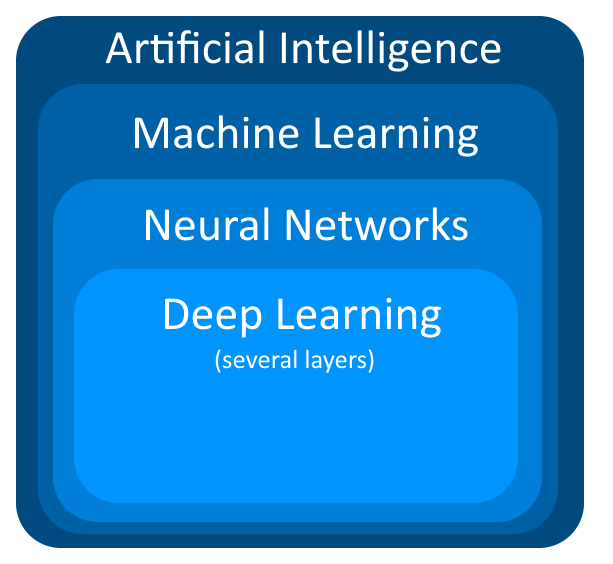
\includegraphics[width=6cm]{resources/ai.png}
	\caption{High level visual representation of what fields there are in the study of AI.}
	\label{fig:ai}
\end{figure}
\subsection{Neural Networks}
The idea of neural networks is not new. In fact, it has been around for decades, but it only really took off in recent years with the emergence of better and more affordable hardware. The basic idea behind the workings of a neural network are quite straight forward. To start off, I must explain what the basic block for a neural network is, a perceptron.
\\\\
A perceptron can be thought of as a node that takes in a weighted sum of its inputs, runs the value through a function (called the activation function) and outputs a value to be used later. The activation function below is a step function that outputs a $1$ if the weighted sum is more than a certain value. The input labelled $1$ in Figure \ref{fig:perceptron} is used to represent a bias $b$ that is always added to the weighted sum before inputting the value into the activation function. Note that the weighted sum can be written in a vectorised format.
$$w \cdot x \equiv \sum_j w_j x_j$$
\begin{eqnarray}
  \mbox{output} = \left\{ 
    \begin{array}{ll} 
      0 & \mbox{if } w\cdot x \leq 0 \\
      1 & \mbox{if } w\cdot x > 0
    \end{array}
  \right.
\end{eqnarray}
\begin{figure}[H]
	\centering
	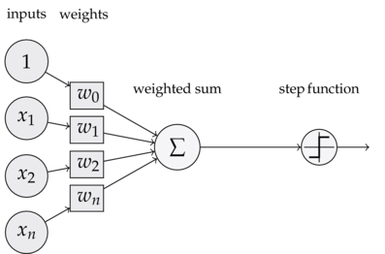
\includegraphics[width=6cm]{resources/perceptron.png}
	\caption{Major components of a perceptron.}
	\textsf{\small (https://blog.knoldus.com/introduction-to-perceptron-neural-network/)}
	\label{fig:perceptron}
\end{figure}
The activation function can be swapped out from the step function that was being used earlier to something else, for instance ReLU (what we will be using) which takes the max of either 0 or the weighted sum.
\begin{eqnarray}
  \mbox{output}&=& \mbox{max}\left\{0,w\cdot x + b\right\}
\end{eqnarray}
In a neural network, there are layers of such perceptrons. Each layer connected to another in a different way. The basic stages are to feed data through to make predictions, compare them with the actual predictions and then use an algorithm called back propagation to update the values of the weights for every perceptron (referred to as nodes from now on). More information on this and the idea of neural networks can be found in the (online) book "Neural Networks and Deep Learning, Michael A. Nielsen"\cite{neuralnets} and the book "Deep Learning with Python, Francois Chollet"\cite{deeplearning}
\subsubsection{Dense Layers}
The way the nodes are connected to each other is called the architecture of the network. Densely connected layers of nodes can be seen in Figure \ref{fig:densenet}. In these, all the nodes are connected to every node in the subsequent layer.
\begin{figure}[H]
	\centering
	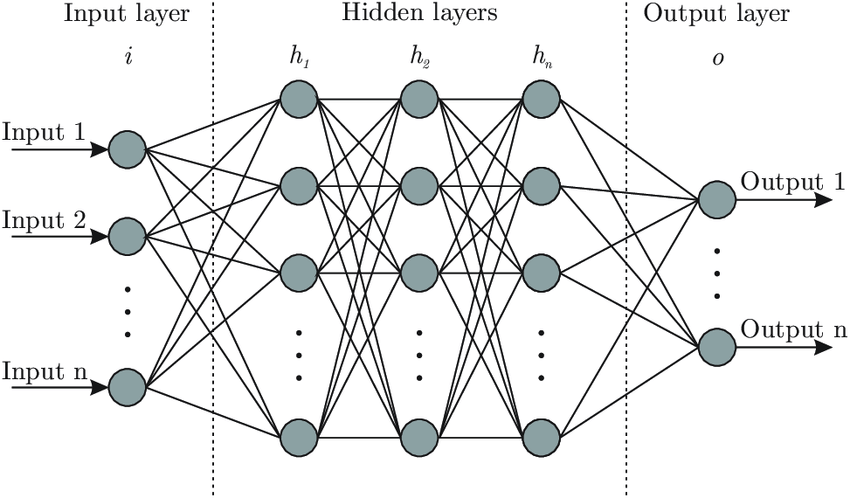
\includegraphics[width=6cm]{resources/densenet.png}
	\caption{Basic neural network architecture\cite{bre2018prediction}.}
	\label{fig:densenet}
\end{figure}
\subsubsection{Convolutional Layers}
These are more complicated than the previously mentioned dense layers. Without going into too much unnecessary details, the basic idea is that the layers in this architecture try to find patterns in the input data and then output the presence of them. 
\\\\
A convolutional layer has a kernel or a window that is used to look over the input data and recognise patterns localised in that window. Every layer has a "depth" number of sub-layers which represent the patterns that the layer is trying to learn and the subsequent layers are connected to these. For instance, with the depth being 3, the convolutional layer looks for 3 patterns in that layer. Figure \ref{fig:convnet} does a good job of giving an idea about how this process works. But the main concept remains the same. There are underlying weights that are being tweaked to learn patterns.
\begin{figure}[H]
	\centering
	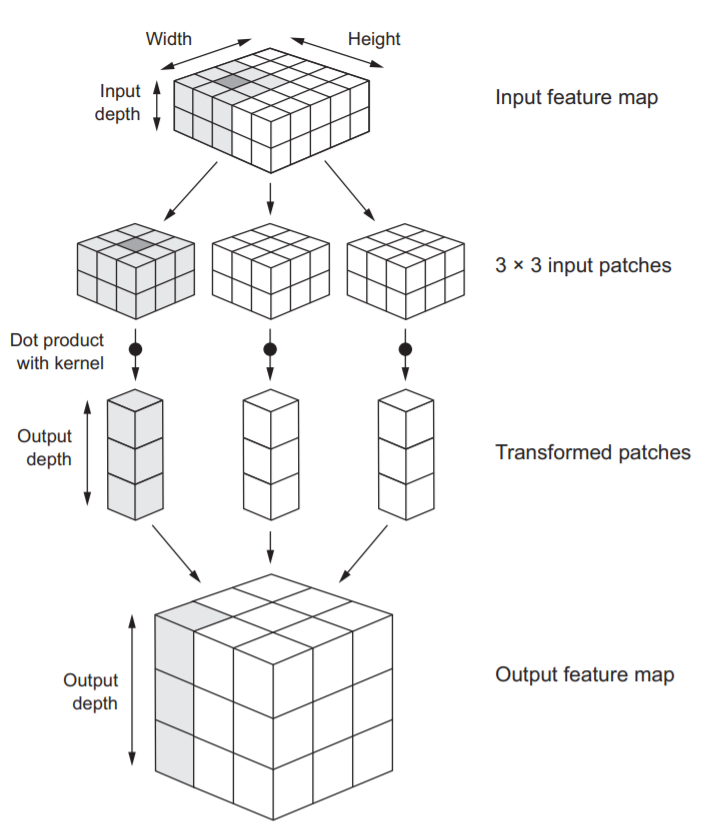
\includegraphics[width=8cm]{resources/convnet.png}
	\caption{How a convolution works\cite[(Page 125, Chapter 5)]{deeplearning}.}
	\label{fig:convnet}
\end{figure}
At the end of a series of convolutional layers, there is a series of dense layers that are used to give the predicted output(s). 
\clearpage



\section{Background}
\subsection{Introduction}
Modern day edge devices have a wealth of data on them and have more than enough computation power to run complex calculations on them with ease. These devices can range from a personal computer to a smart phone. In a world where data is power, access to the data on these devices is highly advantageous.
\\\\
Machine Learning, a branch of Artificial Intelligence (AI), is based on the idea of creating a model that recognises patterns from data to be able to solve prediction problems. To be able to do so effectively, one must have access to a lot of data. More data equates to a higher probability of having a more robust and better overall model. If a model can look and learn from more data, the chances are that it can generalise well, and that is the ideal goal. 
\\\\
The solution to having well trained models seems simple now. Just use the vast amounts data from the edge devices to train a model, correct? To do so, the users must give their data to a server so that the server can then train the model on the data that was just provided to it by the edge users. This trained model can then be used by everyone to predict unseen samples. But what if the users don't want to share their data but still want the benefits of having a model trained on everyone's data?
\subsection{Motivation}
There are numerous instances where people may not want to share their personal data. For instance, for the training of a model that deals with predictive text, the input data would require essentially everything that a user may type into their device. It is pretty obvious to see why some people may not want to share the messages and other content that they type on their devices. It is a clear invasion of their privacy.
\\\\
Another application could be training on images for classification purposes. People may not want to share images, which may include sensitive images, that they have stored on their devices with a third party. This can be extended to an even more sensitive topic of medical imaging where people may not want to share something like the X-Rays of their bodies.
\\\\
In general, people are sceptical of sharing personal data. But we still want to train a model that has had exposure to as much data as possible. Is there a compromise?

\subsection{Federated Machine Learning}
This was the motivation behind the idea of Federated Machine Learning. The idea of privacy, the idea of not having to share your data with someone else and yet still have the benefits of having a model that has exposure to their data.
\\\\
Traditional ML where everyone sends their data to a server, a central user, and the model is trained on everyone's data on the server. In Federated ML, an identical copy of the model is sent to every participating edge user. 
(Section~\ref{sec:ai}) 
\clearpage
\section{Literature Review}
How to train 
Google doing it
Privacy
Federated
Runing on edge too
Differential 

\subsection{What has been done, not mine but others}
\subsection{Google doing it}
\subsection{Privary}
\subsection{Differntial privacy}

\clearpage
\section{How to train}

\clearpage
\section{running on edge}

\clearpage
\section{Core Design}
\subsection{building an desinging this}
\subsection{implemenatation}
\subsection{Global}
\subsection{google implementation}
\subsection{my implementation}
\clearpage
\section{exnteded ideas}
\subsection{Central Server}

\subsubsection{Weighted Average}
\subsubsection{Excluding based on std dev}
\subsubsection{Local only}
\subsection{Peer to Peer}
\subsubsection{Weighted Average}
\subsubsection{Excluding based on std dev}
\subsubsection{Local only}
\subsubsection{testing}
\section{Datasets used}

\clearpage
\section{testing other weights on global data}

\clearpage
\section{tensorflow}

\clearpage
\section{modily}
h5 files
\clearpage
\section{each dataset output experimentation}
artificial users

For each dataset show the otuput we got

\clearpage
\printbibliography[title={Bibliography}]

\end{document}

